%Templated from IEEE Preparation Papers
\documentclass[letterpaper, 10 pt, conference]{ieeeconf}

\IEEEoverridecommandlockouts                              % This command is only
                                                          % needed if you want to
                                                          % use the \thanks command
\overrideIEEEmargins
% See the \addtolength command later in the file to balance the column lengths
% on the last page of the document



%The following packages can be found on http:\\www.ctan.org
\usepackage{graphics} % for pdf, bitmapped graphics files
\usepackage{epsfig} % for postscript graphics files
\usepackage{mathptmx} % assumes new font selection scheme installed
\usepackage{times} % assumes new font selection scheme installed
\usepackage{amsmath} % assumes amsmath package installed
\usepackage{amssymb}  % assumes amsmath package installed



\title{\LARGE \bf
Coding Theory: A Memory Systems Perspective
}

\author{ \parbox{3 in}{\centering Will Wu\\
        Electrical and Computer Engineering\\
        University of Rochester\\
        500 Computer Studies Building \\
        Rochester, NY 14627\\
        {\tt\small ywu37@ur.rochester.edu}}
}

\begin{document}

\maketitle
\thispagestyle{empty}
\pagestyle{empty}


%%%%%%%%%%%%%%%%%%%%%%%%%%%%%%%%%%%%%%%%%%%%%%%%%%%%%%%%%%%%%%%%%%%%%%%%%%%%%%%%
% \begin{abstract}


% \end{abstract}


%%%%%%%%%%%%%%%%%%%%%%%%%%%%%%%%%%%%%%%%%%%%%%%%%%%%%%%%%%%%%%%%%%%%%%%%%%%%%%%%

\section{THE NATURE OF DATA IN COMPUTATION}

The motivation for computing originates from fast data generation and long data retention.  Computing devices are designed to precisely return outputs of functions built from computational primitives given inputs.  Some pieces of data may be reused in the future for a logically sequential computation as part of an algorithm.  This necessitates a device that houses this information for some unknown amount of time for later use.  An entire memory hierarchy This paper will focus on the realm of data storage and the various coding systems implemented to ensure its integrity.  The 

We can generalize all computing down to two tasks: (1)generating data, and (2)storing data for future use.  In the time period between the initial storage of the data and the read request on the data, subatomic particle bombardment such as alpha particle decay cosmic electrical noise denoted as single event upsets can cause bits to flip from one state to the other. \cite{Jacob}   So in that sense, all applications are data sensitive.  The sensitivity level of that data can be directly tied to the tolerance level of users for data error or erasure.  For instance, users accessing a database for has low tolerance while users viewing a picture can tolerate slight imperfections in a subset of the pixels in that picture.  These activities are possible since all data (such as database entries and pictures) reside in some way on some physical medium.

The purpose of memory devices has been made essential and the importance of data integrity has been made.  General protocols for diagnosing singular problem events but very little has been studied about long-term memory device degradation.  Schroeder et al. conducted such a study looking at three sample hard disk drive environments over the course of five years.  The three samples of interest include a high performance computing node (HPC1) and two different web servers from two different internet service providers (COM1) (COM2).  They disclose the costs of maintaining these environments in the following table.  Disk replacement consistently ranks among one of the highest monetary costs.  In the case of HPC1, the workload of computation and virtual simulations allowed for very low error tolerance.  In the case of COM1 and COM2, the high volume workload of web requests also requires low error tolerance.
\begin{figure}[!ht] %Component Replacement
	\centering
	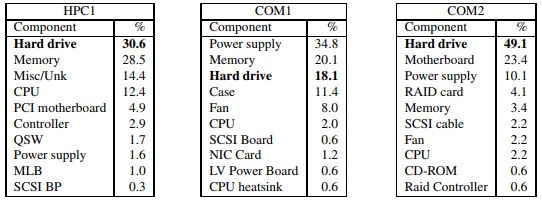
\includegraphics [width=0.5\textwidth] {Component Replacement.JPG} 
    \caption{Component Replacement Data by Monetary Costs.\cite{MTTF Million}}

\end{figure}

\section{THE NATURE OF CODES}

Data is stored in the form of binary digits on random access memory devices and as ferromagnetic polarization in hard disk drives.  The aforementioned bit flipping is one such data error events.  The other event that can occur is bit erasure: where a previous data bit of either '1' or '0' is stored as neither.  A codeword is considered valid if it is a codeword devoid of errors.  An invalid codeword contains some error.  If the codeword is recoverable, we can interpret an invalid codeword as a valid codeword.

In an attempt to improve data integrity, some amount of redundancy must be attached to the codeword.  The simplest method of redundancy is to append one or more duplicate copies of the exact codeword.  Using this method, discrepancies in codewords can be resolved with majority voting or fewest differing bits. \footnote{This metric is called the Hamming distance and will be discussed in the next section.}  The other method of adding redundancy is to not necessarily duplicate the data but to compute parity bits on a subset of the codeword bits, with each parity bit computing a different subset of the codewords bits.  A general rule is that for a codeword of length n, there should be approximately log(n) parity bits.  This corresponds to the logic depth ratio of binary strings.  Most memory devices use parity bits as the error correction codes of choice and is part of the block with the message codeword.  This is done by adding the parity bits to the message codeword either interleaved or on either end of the message codeword.

The bits stored on memory devices can be broken into two pieces: data bits, metadata bits.  In the context of information transfer(R), the addition of these metadata bits decreases the information transfer by the bit ratio that the metadata takes up.

\begin{equation}

R_{with metadata bits} = R * \frac{(Metadata bits + Data bits)}{Metadata bits}

\end{equation}

When a codeword is declared erroneous, there are many aspects of a codeword that can make it so.  The codeword can have multiple bit errors and the location of these errors may not be known. The step past identifying that an error exists in a codeword is correcting the error.  It is important to note the relationship between error detection and error correction.  In order to correct an error, it must be detected.  However, not all detected errors can be corrected.

There are two qualifications of codeword errors in data storage: soft errors and hard errors.  Soft errors can be corrected without notifying the user and as such, do not affect device functionality.  It is the development of these error correction codes that allow for a device to sustain multiple soft errors.  Hard errors appear when a read request is made on the corrupted data and affect device functionality.  Many soft errors over the lifetime of a device can eventually result in a hard error.  Hard errors are irreversible and is caused by the physical properties of the device being altered in some way.  For low error tolerant data applications, it is industry practice to highly prioritize replacement of a memory device after encountering a soft error.\cite{DRAM}  Upon a device encountering a hard error, it is impossible to recover all data from the affected device.  It is however possible to recover a subset of the data on the device and those will typically be physically located in unaffected areas of the device.

\section{CODE ATTRIBUTES}

There are many different aspects of code generation that can be changed to induce different effects.  When discussing varying types of codes, it can be useful to use some notation to concisely offload information about the codes properties.  One such notation (n,k,d)q is used when discussing block codes.

\begin{equation}
(n,k,d)_q
\end{equation}

Where 
\begin{description}
  \item[$\bullet$ ] n denotes the block length
  \item[$\bullet$ ] k denotes the message length
  \item[$\bullet$ ] d denotes the distance
  \item[$\bullet$ ] q denotes the alphabet size
\end{description}

We can represent the space of all codewords with a q-dimension graph with $q^n$ nodes.

The d metric refers to Hamming distance.  This is the number of edges in the graph traversal from one codeword to another codeword.  This is implemented in digital logic using bit-wise XOR between the two codewords and summing the number of '1' bits.  Heuristically, it is assumed that the most likely valid codeword is the one with the shortest Hamming distance to the codeword in question.  If every codeword in the space of all codewords can be corrected to a valid codeword, we call such a code perfect.  However, as the dimensions of n and k increase, the dimension of d scales much less quickly and as a result, there are many codewords that are not recoverable to a valid codeword.  These are the underlying causes of hard errors.

\begin{figure}[!ht]
	\centering
	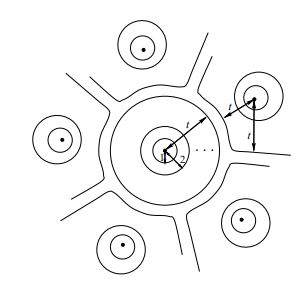
\includegraphics [width=0.5\textwidth] {Hamming Sphere.JPG} 
    \caption{A Visual Representation of a Perfect Hamming Code\cite{McKay}}

\end{figure}

Revisiting our information transfer rate formula, 
\begin{equation}
R_{with metadata bits} = R * \frac{n}{n-k}
\end{equation}

%* Code Generation Matrix and Parity Check Matrix and Galois Field
There are two matrix primitives used to construct parity bits: The generator matrix with dimensions $k$x$n$ and its inverse, the parity check with matrix $(n-k)$x$n$.  The generator matrix is composed of the identity matrix with parity bit assignments (this is denoted by the submatrix P).  Each row of matrix P with dimensions $k$x$k$ denotes a parity bit and its index.  The codeword bits that are used to compute each parity bit are denoted by '1' and those codeword bits omitted are denoted by '0'. 

\begin{equation}
\begin{bmatrix}
    G 
  \end{bmatrix}
  =
  \begin{bmatrix}
    $I_k$ $P$
  \end{bmatrix}
\end{equation}

\begin{equation}
\begin{bmatrix}
    H
  \end{bmatrix}
  =
  \begin{bmatrix}
    $-P^T$ $I_{n-k}$
  \end{bmatrix}
\end{equation}

Since these error correction codes are linear, both code generation matrix G and parity check matrix H can be computed using Galois Field as transforms.  An example of this transform is shown below.  This parity check matrix is constructed in such a way that the codeword matrix and parity matrix have a product of the zero matrix. 

\begin{equation}
\begin{bmatrix}
    G 
  \end{bmatrix}
  \begin{bmatrix}
    $H^T$
  \end{bmatrix}
  =
    \begin{bmatrix}
    I
  \end{bmatrix}
\end{equation}
\begin{equation}
\begin{bmatrix}
    C
  \end{bmatrix}
  \begin{bmatrix}
    $H^T$
  \end{bmatrix}
  =
    \begin{bmatrix}
    0
  \end{bmatrix}
\end{equation}


\begin{figure}[!ht]
	\centering
	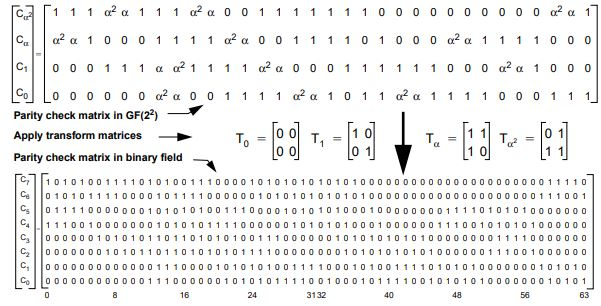
\includegraphics [width=0.5\textwidth] {2-adjacent parity check matrix.JPG} 
    \caption{Formulation of Parity Check Matrix based on Galois Field Transforms.\cite{Jacob}}

\end{figure}


\section{CASE STUDY: ERROR CORRECTION FOUND IN RAM DEVICES}

The ECC discuss above is an attempt at correcting local soft errors in DRAM.  There are some implementations of a protocol to correct errors with the assistance of memory controllers in DRAM devices before they turn into hard errors.  This method is called memory scrubbing and involves transferring block data to memory controllers when the DRAM device is otherwise being idle.  Memory scrubbing allows for multiple errors that span a wide range of addresses and blocks to be corrupted.  There is a tradeoff with using memory scrubbing in terms of the power dissipation with this operation and the high bandwidth stress with transferring data from DRAM to memory controller and back.  Memory scrubbing rates have been reported to be in the neighborhood of 1GB per 45 minutes.\cite{DRAM}

\section{CASE STUDY: B-ADJACENCY ERROR CORRECTION AND CHIPKILL}

Chipkill is a technology that collects the error correction codes of all blocks and adds redundancy to the parity bits by replicating them .  This is redundant duplication of data among multiple separate devices is akin to the redundancy structure of low-level RAID.  The error correction codes in one device can be split in half and that half sent to a neighboring DIMM device.  The DIMM will receive half of the error correction codes from a different DIMM device.  This striation of error correction codes allow for error correction codes of neighboring block codes to be found in physically distant DIMM devices.  This allows for errors of more distant bits to be correctable.  As b cycles of error code striations occur, errors with distance b apart are correctable.  The primary tradeoff of this method is the high redundancy in the error correction codes among DIMM devices.  There is a high space cost associated with this technique.

\begin{figure}[!ht]
	\centering
	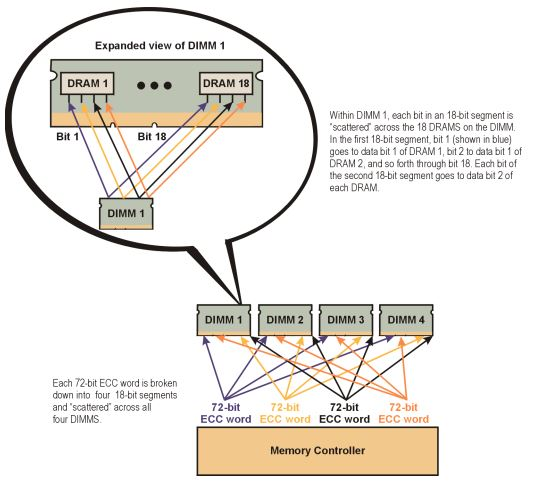
\includegraphics [width=0.5\textwidth] {ChipKill.JPG} 
    \caption{ChipKill implementation on Dell PowerEdge 6000 series servers.\cite{Chipkill}}

\end{figure}

\section{CASE STUDY: REED-SOLOMON CODING}

We have already discussed how the code generation matrix and parity check matrix can be formulated and how it aids in generating parity bits for error correction coding.  \cite{Reed-Solomon} In Reed-Solomon codes, the message codeword is put into matrix form (denoted by matrix C) to align with the dimensions of its code generation matrix.  This makes it so that the message codewords along the diagonal of the identity matrix are retained while the parity bits are computed.  Using the inverse properties of the code generation matrix and parity check matrix, we can recover erroneous codewords by anticipating the product of G*C*$H^T$ to have an identity matrix diagonal with zero values everywhere else.

This code is part of the BCH cyclic codes and is one of the strongest error correction schemes.  With the use of Reed-Solomon and adequate block content striping, up to (n-k)/2 bits of the block can be corrupted or erased and can still be recovered. \cite{Secret Share}  This is done using the uncorrupted data and the aforementioned parity check matrix and code generation matrix.  This coding mechanism is utilized in RAID6 disk drive technologies and its main improvement over RAID5 is its ability to recover multiple from non-adjacent bit errors.



\addtolength{\textheight}{-12cm}   % This command serves to balance the column lengths
                                  % on the last page of the document manually. It shortens
                                  % the textheight of the last page by a suitable amount.
                                  % This command does not take effect until the next page
                                  % so it should come on the page before the last. Make
                                  % sure that you do not shorten the textheight too much.


\begin{thebibliography}{99}

\bibitem{MDS} Blaum, Mario, James Lee Hafner, and Steven Hetzler. "Partial-MDS Codes and Their Application to RAID Type of Architectures." IEEE Trans. Information Theory 59.7 (2013): 4510-4519.​

\bibitem{b-Adjacent} Bossen, D. C. "b-Adjacent error correction." IBM Journal of Research and Development 14.4 (1970): 402-408.​

\bibitem{Reed-Solomon} Dau, Hoang, et al. "Repairing Reed-Solomon codes with multiple erasures." IEEE Transactions on Information Theory(2018).​

\bibitem{Chipkill} Dell, "A White Paper on the Benefits of Chipkill-Correct ECC for PC Server Main Memory," IBM Microelectronics Division (July 1997),​

\bibitem{Jacob} Jacob, Bruce, Spencer Ng, and David Wang. Memory systems: cache, DRAM, disk. Morgan Kaufmann, 2010.​

\bibitem{Huffman} Huffman, W. Cary, and Vera Pless. Fundamentals of error-correcting codes. Cambridge university press, 2010.​

\bibitem{MacKay} MacKay, David JC, and David JC Mac Kay. Information theory, inference and learning algorithms. Cambridge university press, 2003.

\bibitem{Secret Share} McEliece, Robert J., and Dilip V. Sarwate. "On sharing secrets and Reed-Solomon codes." Communications of the ACM 24.9 (1981): 583-584.

\bibitem{Maximum Likelihood} Miller, Gadi, and David Burshtein. "Bounds on the maximum-likelihood decoding error probability of low-density parity-check codes." IEEE Transactions on Information Theory 47.7 (2001): 2696-2710.​

\bibitem{MTTF Million} Schroeder, Bianca, and Garth A. Gibson. "Disk failures in the real world: What does an mttf of 1, 000, 000 hours mean to you?." FAST. Vol. 7. No. 1. 2007.​

\bibitem{DRAM} Schroeder, Bianca, Eduardo Pinheiro, and Wolf-Dietrich Weber. "DRAM errors in the wild: a large-scale field study." ACM SIGMETRICS Performance Evaluation Review. Vol. 37. No. 1. ACM, 2009.

\bibitem{Tanner} Tanner, “A recursive approach to low-complexity codes,” IEEE Trans. Inform. Theory
IT–27 (1981), 533–547.

\bibitem{Wikipedia} https://en.wikipedia.org/wiki/Parity-check-matrix

\end{thebibliography}

\end{document}
